% Link to template used: https://de.overleaf.com/project/5ede5800d140f800011e23ed
%=================================================================
\documentclass[journal,article,processes,submit,moreauthors,pdftex]{Definitions/mdpi} 


%=================================================================
\firstpage{1} 
\makeatletter 
\setcounter{page}{\@firstpage} 
\makeatother
\pubvolume{xx}
\issuenum{1}
\articlenumber{5}
\pubyear{2020}
\copyrightyear{2020}


%=================================================================
% Add packages and commands here. The following packages are loaded in our class file: fontenc, calc, indentfirst, fancyhdr, graphicx, lastpage, ifthen, lineno, float, amsmath, setspace, enumitem, mathpazo, booktabs, titlesec, etoolbox, amsthm, hyphenat, natbib, hyperref, footmisc, geometry, caption, url, mdframed, tabto, soul, multirow, microtype, tikz

% Own added packages
\usepackage{textcomp}
\usepackage{makecell}
\renewcommand\cellalign{tl}
\usepackage{ulem}
\usepackage{gensymb}
\usepackage{wrapfig}
\usepackage{subcaption}

%=================================================================
% Full title of the paper (Capitalized)
\Title{3D-Druck in der Verfahrenstechnik, Designing a induction heat-exchanger for 3D-Printing}

% Author Orchid ID: enter ID or remove command
\newcommand{\orcidauthorA}{0000-0000-000-000X} % Add \orcidA{} behind the author's name

% Authors, for the paper (add full first names)
\Author{Janick Beck and Shukang Zhang}

% Authors, for metadata in PDF
\AuthorNames{Janick Beck and Shukang Zhang}


% Affiliations / Addresses (Add [1] after \address if there is only one affiliation.)
\address{%
}

% Contact information of the corresponding author
\corres{}

% Current address and/or shared authorship
\firstnote{} 
\secondnote{}

% Abstract (Do not insert blank lines, i.e. \\) 
\abstract{}

% Keywords
\keyword{3D-Printing, FLM, AMIR, Mixing Reactor, Induction}

%%%%%%%%%%%%%%%%%%%%%%%%%%%%%%%%%%%%%%%%%%
\begin{document}
%%%%%%%%%%%%%%%%%%%%%%%%%%%%%%%%%%%%%%%%%%

%%%%%%%%%%%%%%%%%%%%%%%%%%%%%%%%%%%%%%%%%%
\section{Introduction}

Additive Manufacturing, AM, is in fact not a new concept. It can track back to 150 years ago, when people used two-dimensional layer overlays to form three-dimensional topographic maps. During the 1960s and 1970s came the first AM-Technology, include photopolymerization technology, Powder fusion in 1972 and sheet lamination in 1979. But at that time, it has no commercial market at all and very few investment in research and development. \cite{link-1}
The first 3D printer, which used the stereolithography technique, was created by Charles W. Hull in the mid-1980s. \cite{link-2}

After 30 years development, 3D Printng has come into personal home. The price is nowadays down to 300 dollars.3D Printing, as a bottom-up-process, has many advantages. With 3D printing, designers have the ability to quickly turn concepts into 3D models or prototypes, and implement rapid design changes. It makes development so much easier, quicker and cheaper. 

Generally, development steps look like this: 
\begin{enumerate}
    \item Identification of project requirements
    \item Computer-aided 3D Model design
    \item Simulation of the 3D Model in corresponding physical field
    \item Optimize according to the results from Simulation
    \item Print real 3D Model via 3D Printing and do experiment
    \item Optimize according to the results from experiment
\end{enumerate}


In this project we will show you how to combine Computer-aided 3D Printing technologies with simulation and data processing to achieve our goal.
 
%%%%%%%%%%%%%%%%%%%%%%%%%%%%%%%%%%%%%%%%%%
\section{Problem}
In our project we have a pipe (Material: Polymer) up to 300mm long, with a internal diameter of 94 mm. A static heat-exchanger need to be built inner the pipe, so that 10[℃]water flow from one side and left the other side 80 \textdegree{}C$\pm$ 5 \textdegree{}C the temperature distribution should be evenly along radial direction. Fluid volume is given with 0.5 $m^3/h$. As thermal source we have chosen electromagnetic induction. To check the temperature along the pipe, we have chosen an infrared thermometer. And another important parameter that need to be confirmed in the experiment is the press-drop. 


%%%%%%%%%%%%%%%%%%%%%%%%%%%%%%%%%%%%%%%%%%
\section{Solution}

\subsection{CAD-Model}

\begin{wrapfigure}{l}{0.3\textwidth}
\centerline{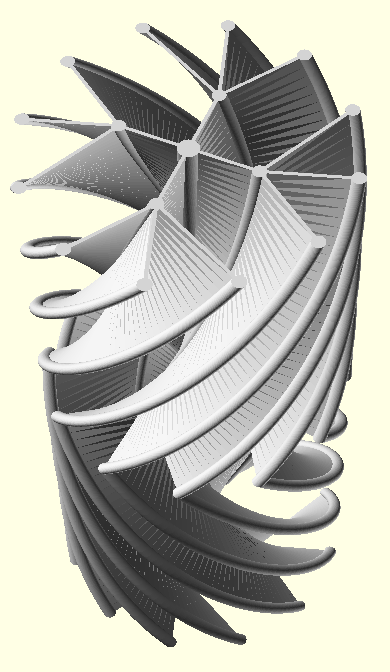
\includegraphics[height=0.48\textwidth]{./docu_pictures/simple_double_part.png}}
\caption{Example CAD model}
\label{cad-number-of-objects}
\end{wrapfigure}

The idea is to create a helical structure with high parameterizability. The helical structure is chosen for it's ability to create a vortex at the outlet and thereby creating a higher mixing of the liquid in the pipe. 

The structure is first created as a two-dimensional drawing which is linearly extruded with a twist. This drawing consists of a number of rings around the center, each containing a certain number of circles. These circles are connected by the shortest path with a circle in the next inner ring. The circles in the innermost ring are connected with the closest other circle from this ring.

This construction allows for the following parameters to be easily changed: Number and distance from center of the rings, number of circles for each ring, twist and the thickness of the edges between the circles. All of those parameters together allow for the structure to have a different density dependent on the distance from the center, thereby being adaptable to the requirements of electrical induction.

After the first simulations it was clear that the structure needs to be longer to have more mass and create more area to transfer the heat. So the structure was mirrored at the top to double it's length and mix the liquid further within the structure with the change in the twist direction.

The CAD modelling script language OpenSCAD \cite{openscad} was used to create STL files of the model together with Python \cite{python} scripts for batch file generation in the design study.

\subsection{Computational Fluid Dynamics(CFD) simulation with Siemens Star-CCM+}
Simulation is a powerful tool to check the quality of the designed system and help to optimize the model and the process. 

Here in our project it is about Computational fluid dynamics simulation that combines fluid with solid. 

\begin{figure}
\begin{center}
\centerline{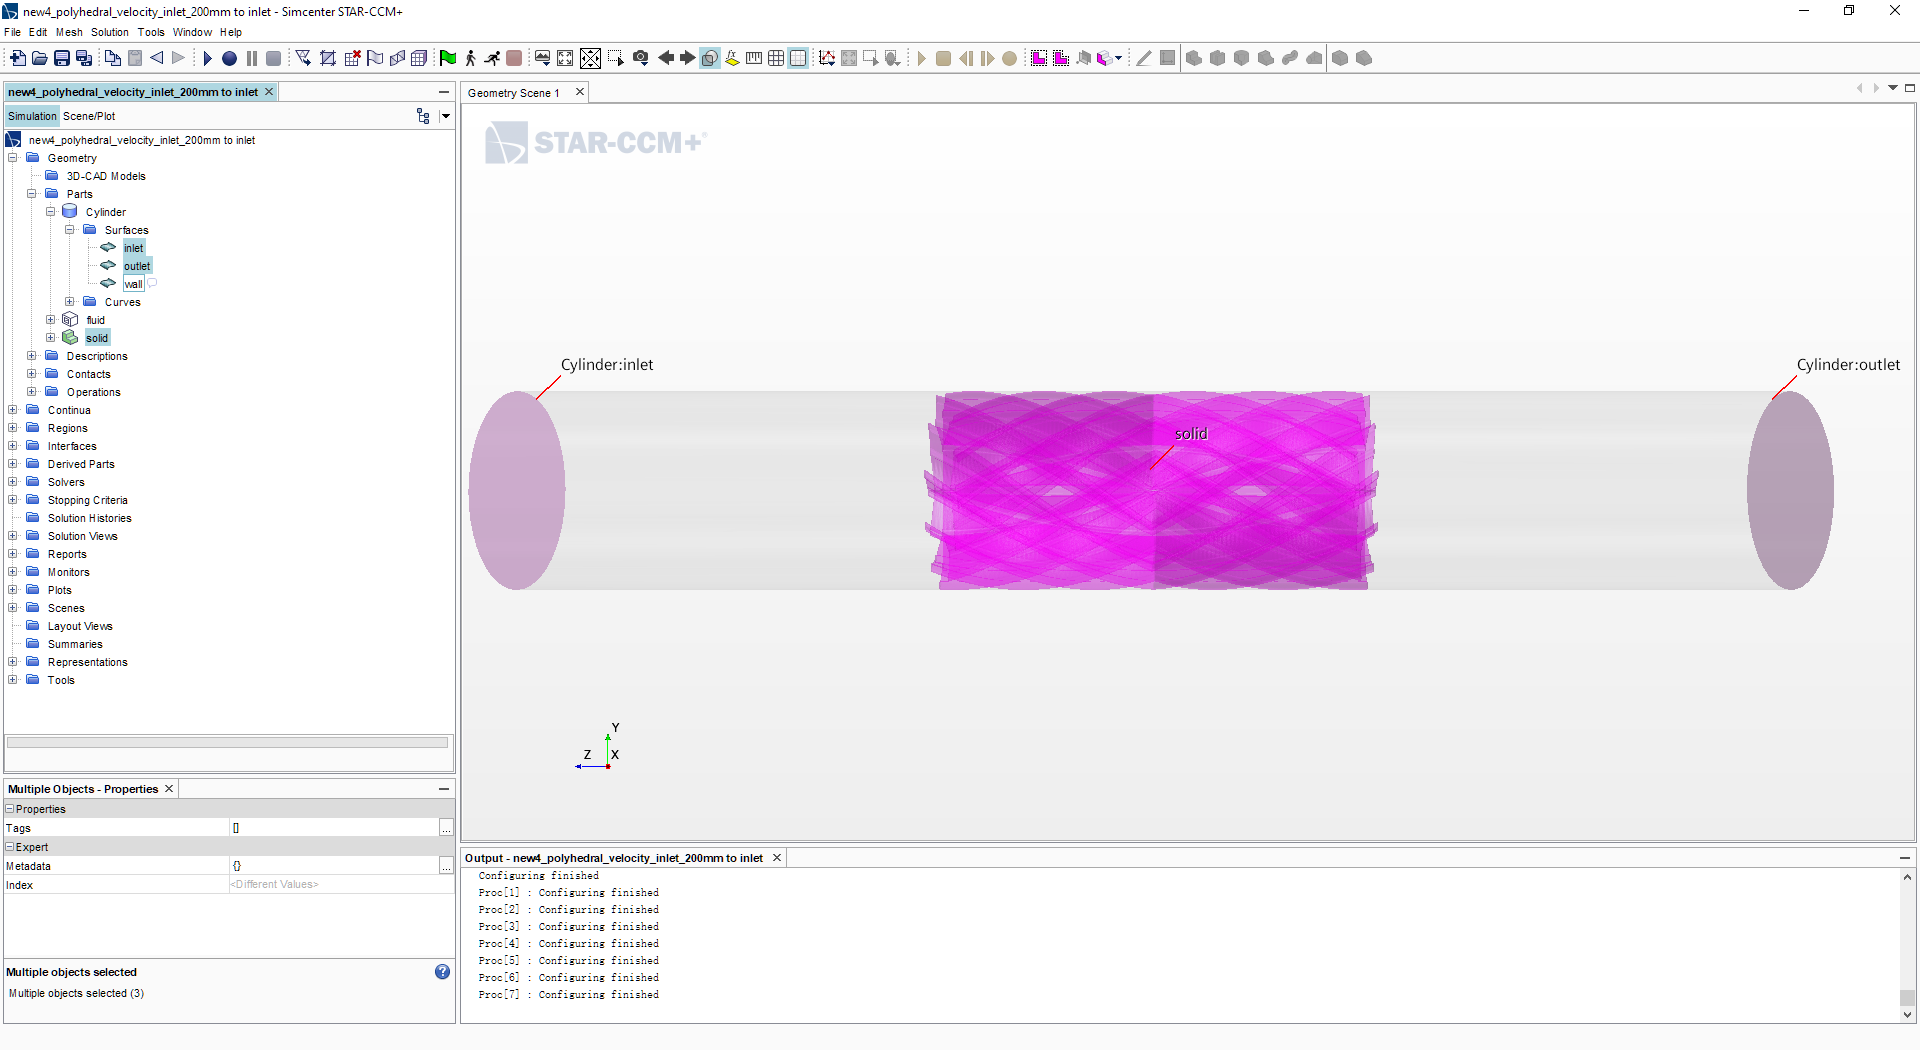
\includegraphics[width=\textwidth]{./docu_pictures/sketch1.png}}
\end{center}
\caption{Geometric view of the simulation. Static heat-exchanger in the middle.}
\label{simulation-sketch}
\end{figure}

When man run a CFD-simulation, the first thing to think about is, that the fluid behaviors laminar or turbulent. First we take a look at a much easier system, water flows direct through the pipe without mixer. Then we can easily calculate the Reynolds number. 

\begin{align*}
    \text{Re} = \frac{\rho ud}{\mu}
\end{align*}

$\rho$ represents the density of the water, $u$ represents the velocity of the water normal to the inlet-surface(see figure 3-1), $\mu$ represents dynamic viscosity of the water, and d the characteristic length, here i.e. the inner diameter $d=0.09$[m]. In this case we have fluid volume of $V = 0.5$ [$\frac{m^3}{s}]=1.389*10^{-4}$ [$\frac{m^3}{s}]$, $\rho_{283K}=999$[$\frac{kg}{m^3}$], $\mu_{283K}=1.3077*10^{-3}$[Pa*s]. The value of the dynamic viscosity of water comes from literature \cite{link-3}. So we get the result $Re_{283K}=1437$.The critical $Re$ value for a laminar fluid in a pipe is 2320 \cite{script}. Then in order to obtain the press drop when water flows through the empty pipe, we run the simulate under laminar model. Under is the software settings as show in Fig. \ref{fluid-settings}. 

\begin{figure}
\begin{center}
\centerline{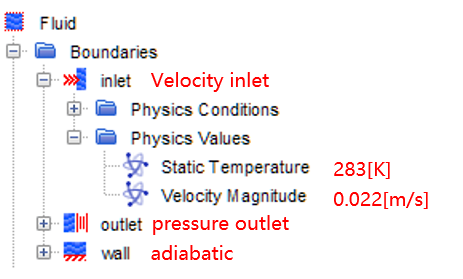
\includegraphics[width=0.4\textwidth]{./docu_pictures/fluid.png} 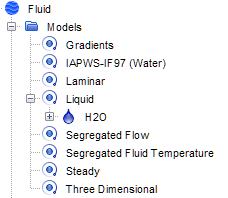
\includegraphics[width=0.4\textwidth]{./docu_pictures/fluid2.png}}
\end{center}
\caption{Simulation fluid settings}
\label{fluid-settings}
\end{figure}

Simulation shows a result of 0.16619[Pa]. This simulation was also run again under same settings except that laminar model changed into turbulent model. And we got a result of 0.16722[Pa]. Almost the same result. Later we will compare these results with the results from experiments. 

Now we can add the mixer into the pipe. This has influence to the characteristic length. Since the definition for the d is:

\begin{align*}
    d \equiv 4 \cdot \frac{\text{fluid passed surface}}{\text{wetted circumference}}
\end{align*}

So the adding of the mixer will reduce the characteristic length and lead to the reducing of Re. But on the other hand, we want to heat the water from 10[℃] to 80[℃], increasing temperature will reduce the dynamic viscosity very obviously. Under 80[℃] is  $\mu_{353K}=0.3565*10^{-3}[\text{Pa}*s]$, and then $Re_{353K}=5272$ when it flows through empty pipe. And $\kappa-\epsilon$-turbulence model, which uses Reynolds-Averaged Navier-Stokes-Equation (RANS), include extra terms to describe the disturbance from environment, that cannot be found in normal Navier-Stokes-Equation. So it's obviously better to run our simulation under turbulent model when we add mixer and thermal source. The software settings are shown in Fig. \ref{software-settings}.

\begin{figure}
\begin{center}
\centerline{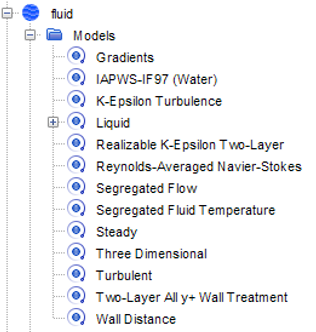
\includegraphics[width=0.3\textwidth]{./docu_pictures/software1.png} 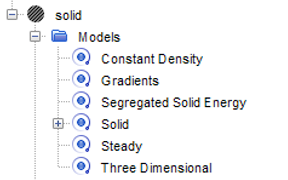
\includegraphics[width=0.3\textwidth]{./docu_pictures/software2.png}
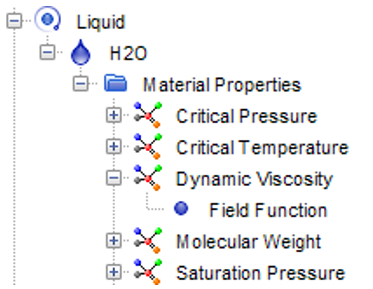
\includegraphics[width=0.3\textwidth]{./docu_pictures/software3.png}}
\end{center}
\caption{Simulation software Settings}
\label{software-settings}
\end{figure}

We use the equation from literature[3] to describe the change of the dynamic viscosity of the water: 
\begin{align*}
    \mu=A*10^{\frac{B}{T-C}}
\end{align*}

Where $A=2.414*10^{-5}[Pa*s]$; $B=247.8[K]$; $C=140[K]$.

\begin{figure}
\begin{center}
\centerline{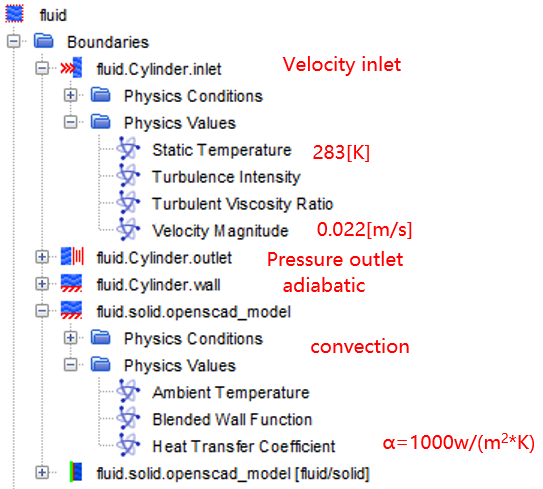
\includegraphics[width=0.3\textwidth]{./docu_pictures/solid1.png} 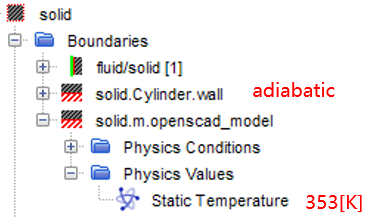
\includegraphics[width=0.3\textwidth]{./docu_pictures/solid2.png}}
\end{center}
\caption{Simulation solid settings}
\label{solid-settings}
\end{figure}

We plan to use the electromagnetic induction method to heat the water, but in order to simplify the simulation. We give here the mixer a steady temperature of 90℃. as shown in  Fig. \ref{solid-settings}.The heat transfer coefficient between mixer and water is given by 1000[$\frac{W}{m^{2}*K}$]. It's a typical value from literature \cite{uebergang-fluessigkeit}. With this base simulation a design study with 216 different CAD-models was conducted.

After generating mesh using polyhedral cell we obtain for fluid 6784729 cells and for solid 3429631 cells, which should be far enough for accurate results. Pictures of the mesh are shown in Fig. \ref{mesh-pictures} and the results in Fig. \ref{vertical-result-pictures}, Fig. \ref{outlet-result-pictures}.

\begin{figure}
\begin{center}
\centering
\begin{subfigure}{1.0\textwidth}
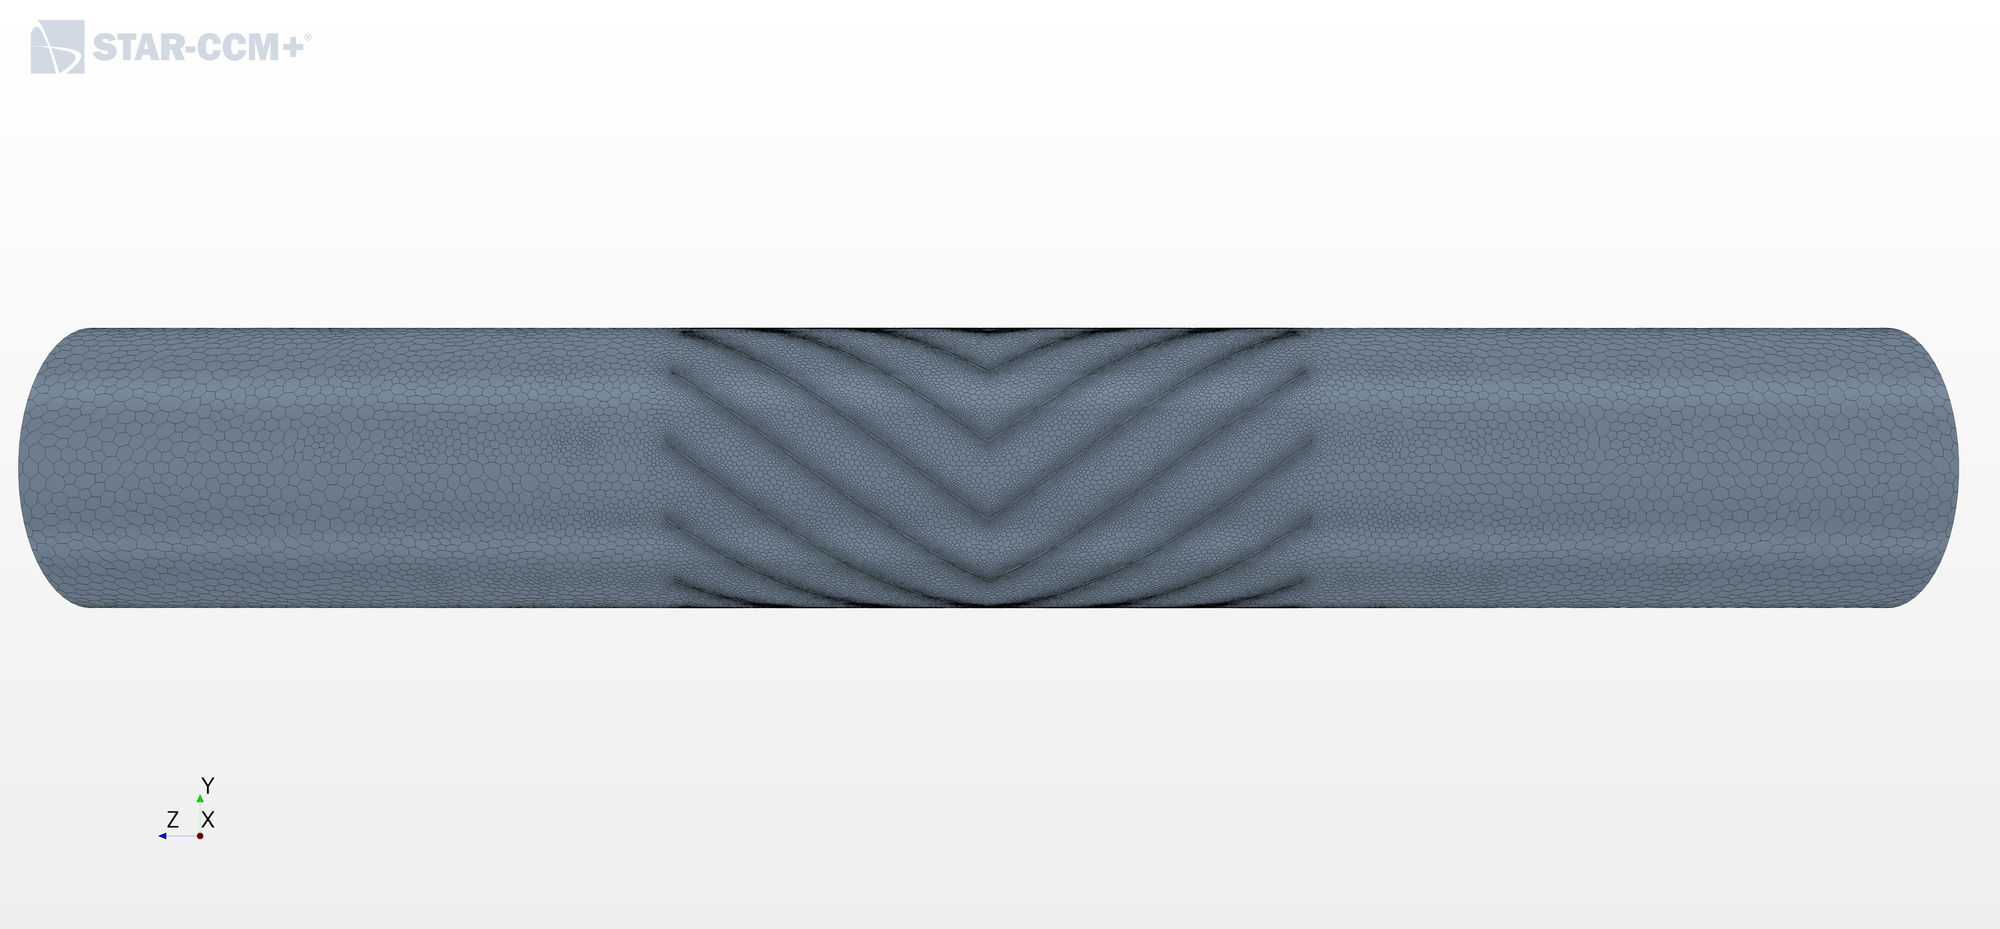
\includegraphics[width=\linewidth]{./docu_pictures/model1.png}
\end{subfigure}
\begin{subfigure}{1.0\textwidth}
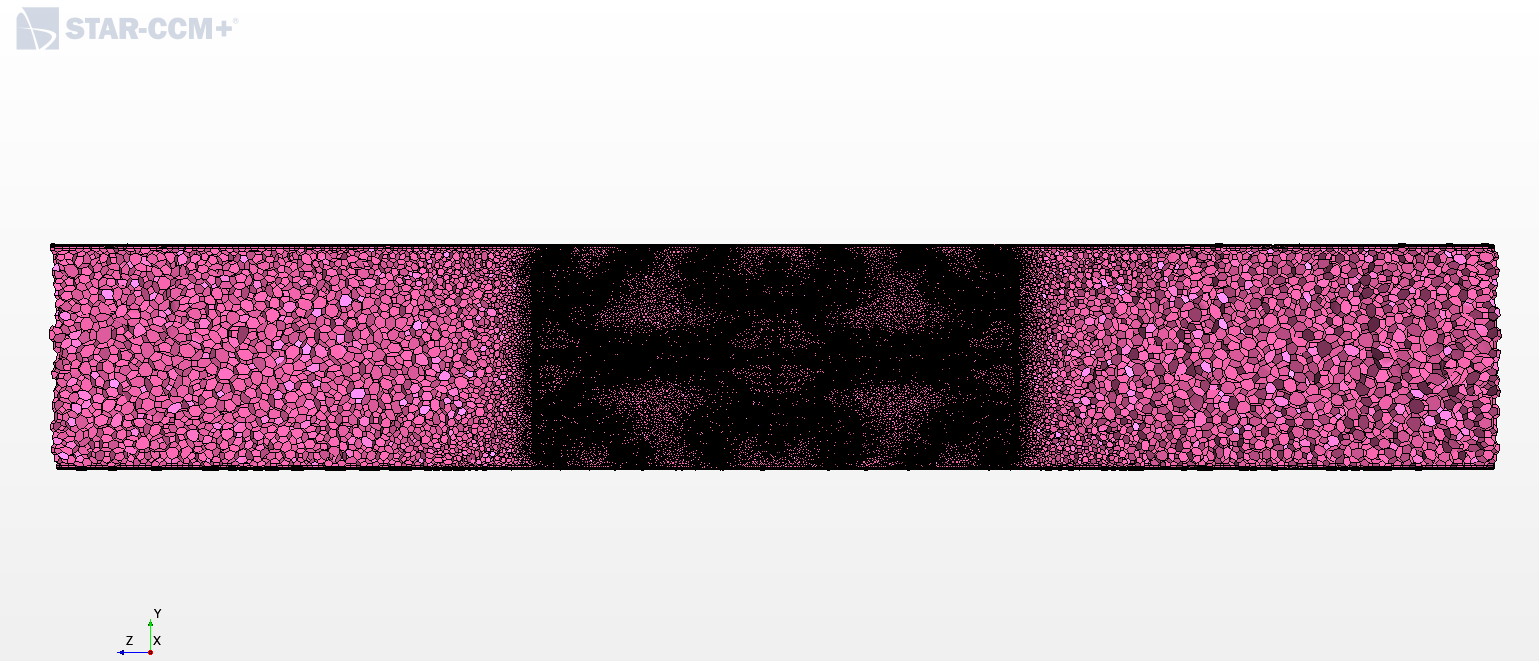
\includegraphics[width=\linewidth]{./docu_pictures/model2.png}
\end{subfigure}
\end{center}
\caption{Mesh view of the model}
\label{mesh-pictures}
\end{figure}

\begin{figure}
%\captionsetup[subfigure]{labelformat=empty}
\begin{center}
\centering
\begin{subfigure}[b]{1.0\textwidth}
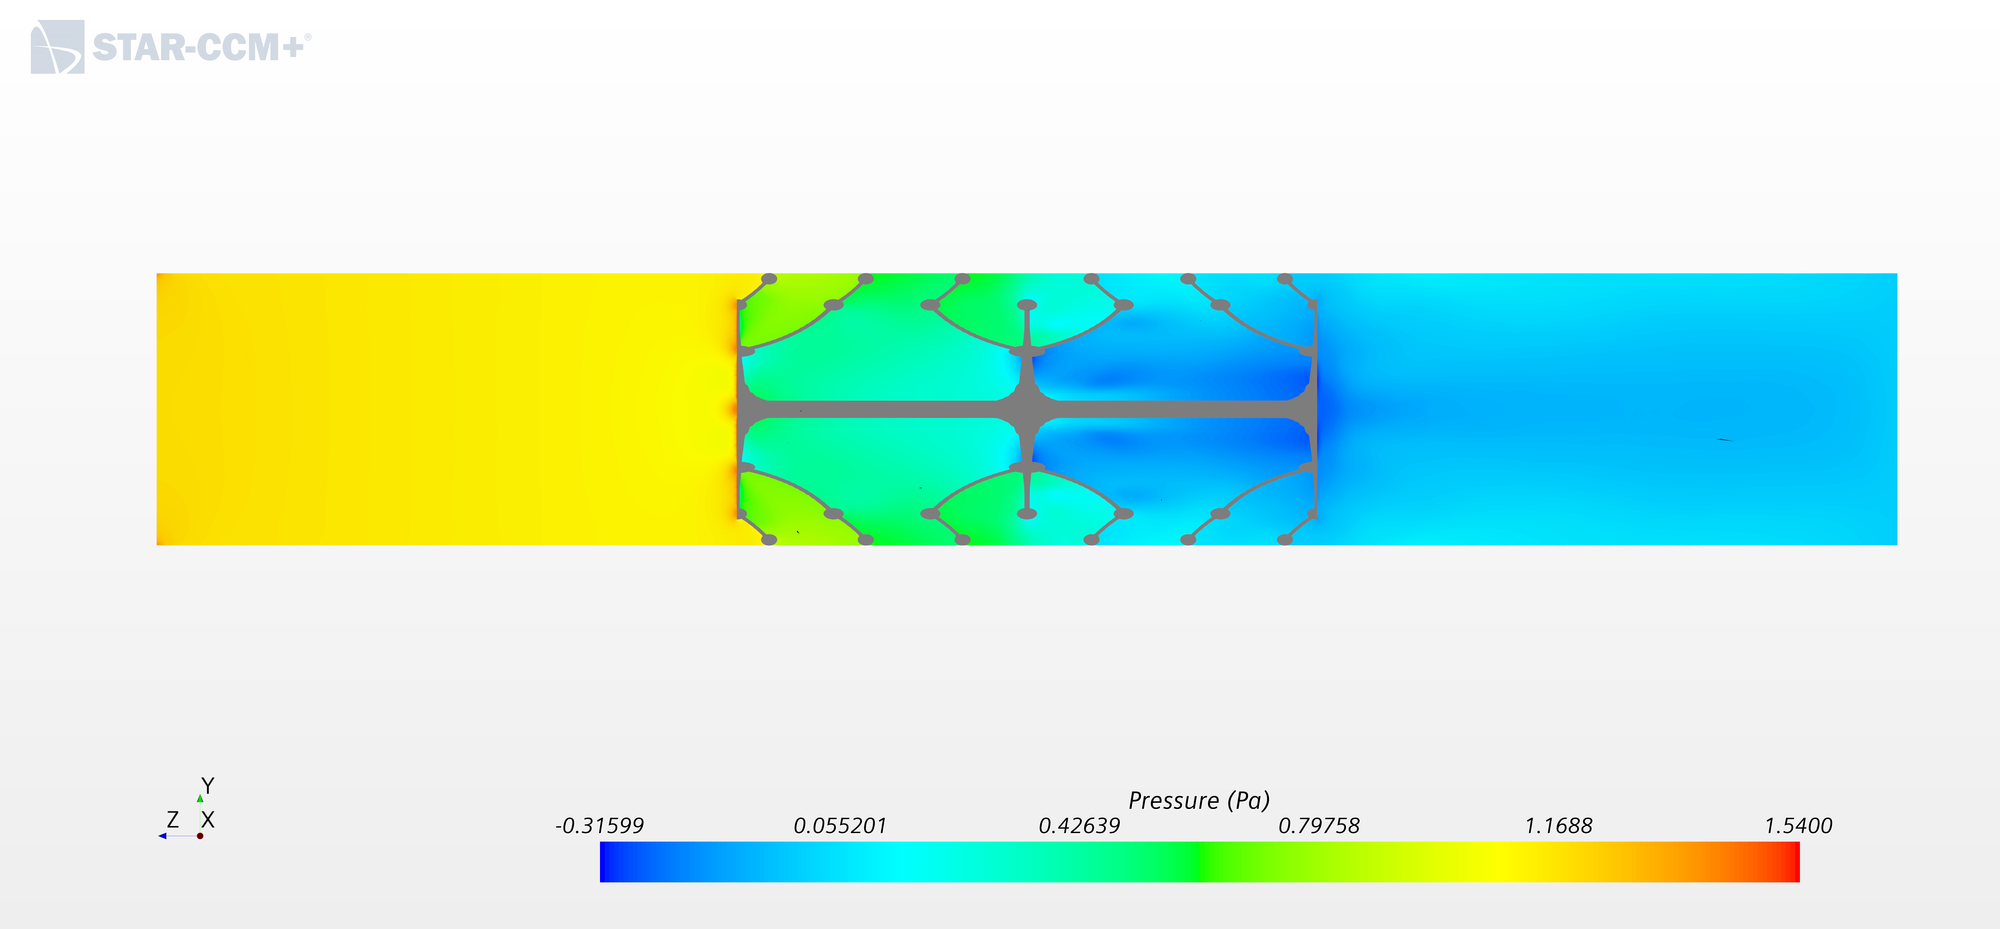
\includegraphics[width=\linewidth]{./docu_pictures/result1.png}
\caption*{The press drop between inlet and outlet is 1.19[Pa]. \\ \vspace{1cm}}
\end{subfigure}
\begin{subfigure}[b]{1.0\textwidth}
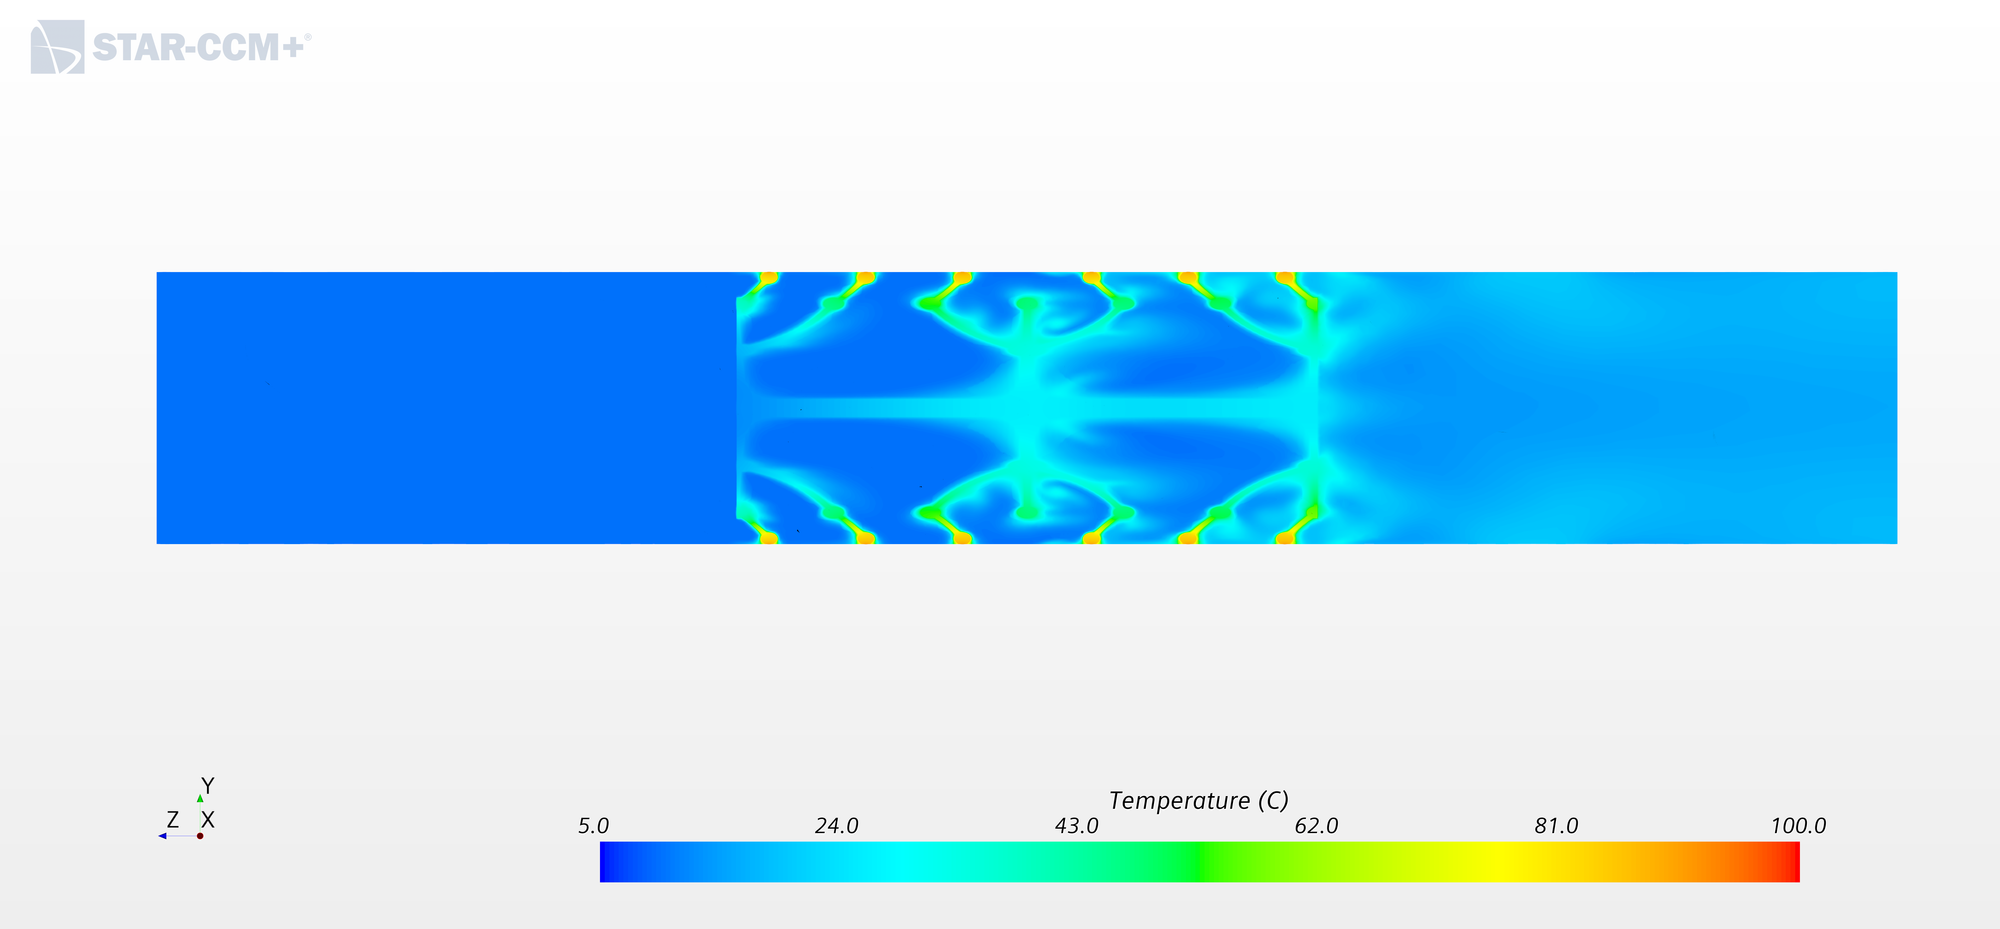
\includegraphics[width=\linewidth]{./docu_pictures/result2.png}
\caption*{The picture above shows temperature distribution along the pipe. It's clear, that water obtain heat from the mixer, because the color change near the interface between the water and the mixer shows obvious temperature gradient. \\ \vspace{1cm}}
\end{subfigure}
\end{center}
\caption{Side view of the results}
\label{vertical-result-pictures}
\end{figure}

\begin{figure}
%\captionsetup[subfigure]{labelformat=empty}
\begin{center}
\centering
\begin{subfigure}[b]{1.0\textwidth}
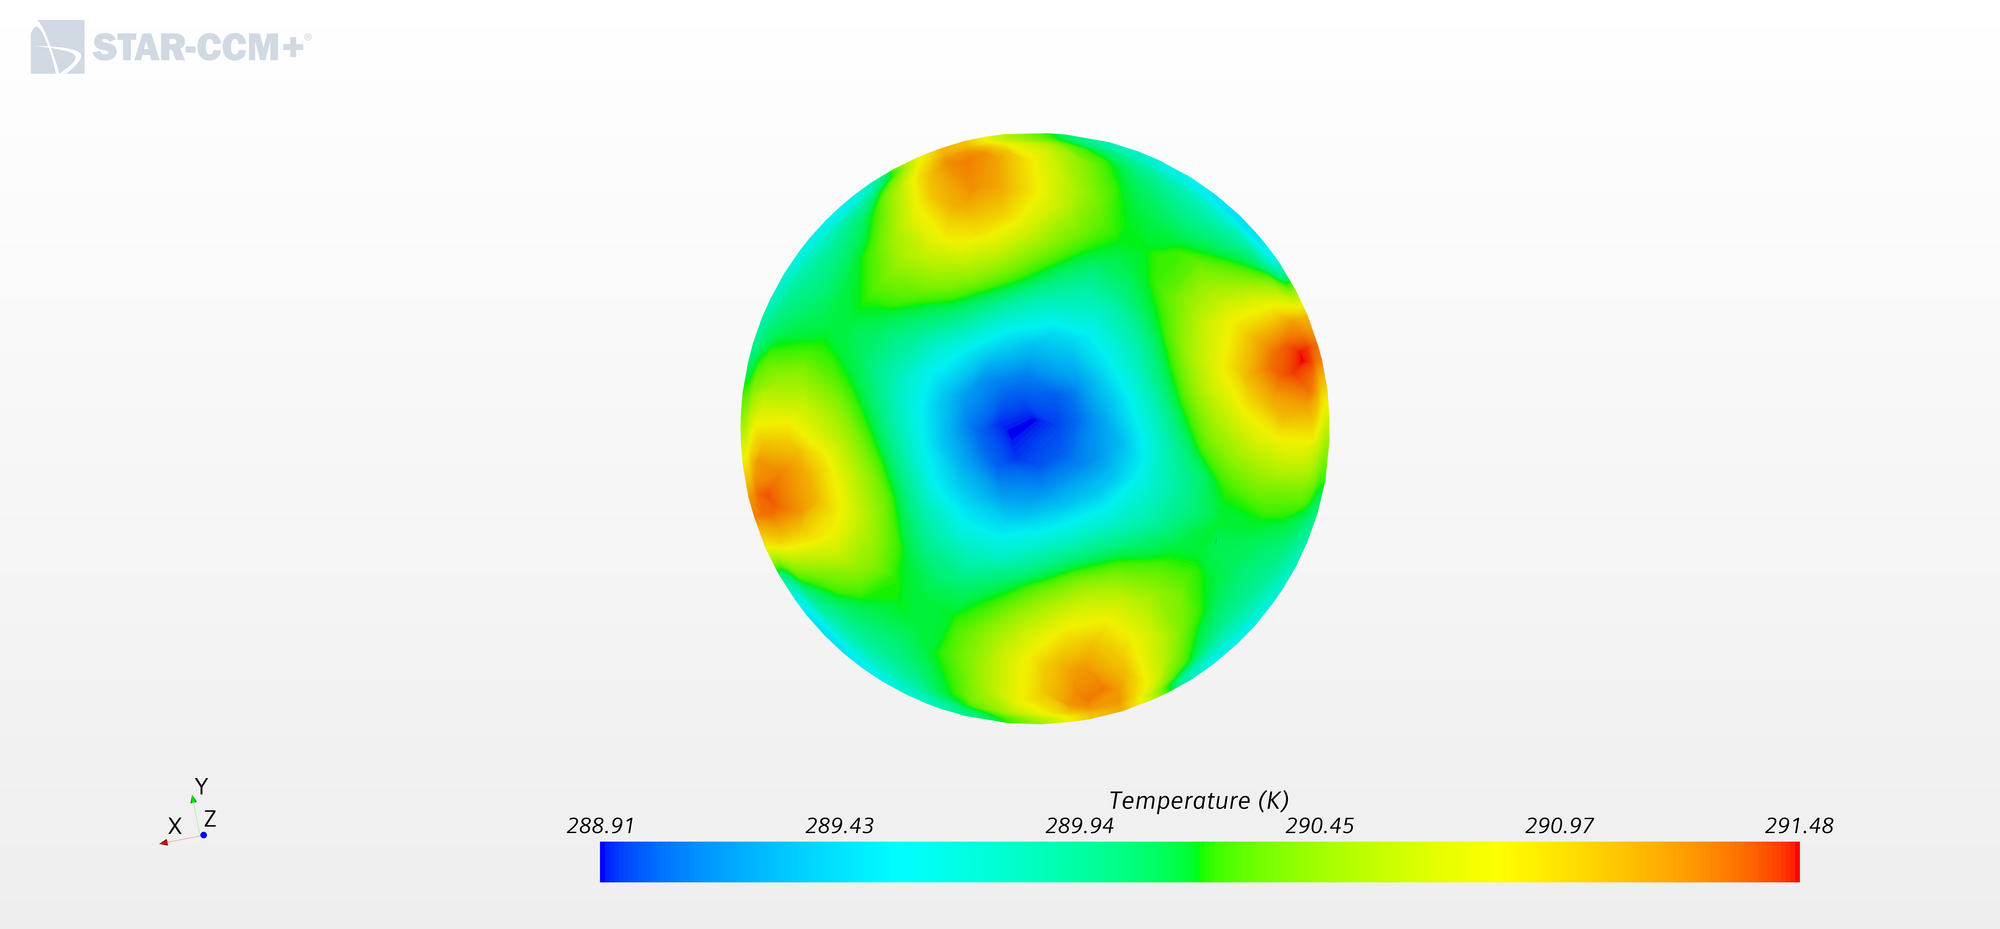
\includegraphics[width=\linewidth]{./docu_pictures/result3.png}
\caption*{Average temperature of the outlet is 17.045[℃], i.e. 290.045[K]. Standard temperature deviation at the outlet is 0.575[℃], which smaller than 1[℃]. Almost a evenly distribution along radial direction.}
\end{subfigure}
\end{center}
\caption{Outlet view of the results}
\label{outlet-result-pictures}
\end{figure}


%%%%%%%%%%%%%%%%%%%%%%%%%%%%%%%%%%%%%%%%%%
\section{Conclusions}

The temperature increases only 7[K] after passing the mixer, which is far away from what was required. But in the future this results can be improved. For example, change the geometry of the mixer to increase the heat exchange. The heat exchange based on contact between fluid element is almost steady and slow, but we can enhance the convection to increase the heat exchange based on material transport and diffusion. So we need to improve the degree of turbulence. 

On the other hand, we can slow down the fluid velocity, so that the fluid element have more time to exchange heat. 

At last, we can also increase the solid temperature, so that water get more heat under the same contact time. But this could lead to higher pressure when the liquid starts evaporating along the mixer.

%%%%%%%%%%%%%%%%%%%%%%%%%%%%%%%%%%%%%%%%%%
\vspace{6pt} 


%%%%%%%%%%%%%%%%%%%%%%%%%%%%%%%%%%%%%%%%%%
%% optional
\abbreviations{The following abbreviations are used in this manuscript:\\

\noindent 
\begin{tabular}{@{}ll}
MDPI & Multidisciplinary Digital Publishing Institute\\
DOAJ & Directory of open access journals\\
TLA & Three letter acronym\\
LD & linear dichroism
\end{tabular}}

%%%%%%%%%%%%%%%%%%%%%%%%%%%%%%%%%%%%%%%%%%
%% optional
\appendixtitles{yes} %Leave argument "no" if all appendix headings stay EMPTY (then no dot is printed after "Appendix A"). If the appendix sections contain a heading then change the argument to "yes".
\appendix
\section{Requirement Specification}
% \usepackage{booktabs}


\begin{table}[H]
\centering
\caption{Requirement specification list for the heat exchanger}
\begin{tabular}{llll} 
\toprule
\begin{tabular}[c]{@{}l@{}}\textbf{Obligatory}\\\textbf{or Desirable} \end{tabular} & \textbf{Category} & \textbf{Description}            & \textbf{Value}          \\ 
\midrule
Obligatory                                                                          & Performance       & volume flow rate                & greater 0.5 m$^3$/h     \\
Obligatory                                                                          & Performance       & heat distribution               & radial and evenly       \\
Obligatory                                                                          & Performance       & heating water flowing trough    & from 10 °C to 80 °C     \\
Obligatory                                                                          & Performance       & low pressure drop               &                         \\
Obligatory                                                                          & Material          & material temperature resistance & between 0 °C and 90 °C  \\
Obligatory                                                                          & Material          & material water solvability      & unsolvable in water     \\
Obligatory                                                                          & Material          & electrical conductivity         & greater $10^6$ S/m      \\
Obligatory                                                                          & Manufacturing     & manufacturing process           & additive manufacturing  \\
Desirable                                                                           & Geometry          & customizability of model        & model is parameterized  \\
Obligatory                                                                          & Geometry          & outer Shape                     & cylindrical             \\
Obligatory                                                                          & Geometry          & outer diameter                  & 94 mm                   \\
Desirable                                                                           & Geometry          & length                          & up to 300 mm            \\
Obligatory                                                                          & Geometry          & outer wall                      & closed                  \\
Desirable                                                                           & Geometry          & outer wall thickness            & smaller 5 mm            \\
Obligatory                                                                          & Geometry          & water flow direction            & fixed direction         \\
\bottomrule
\end{tabular}
\end{table}

\section{Simulation Model Requirement Specification}
% \usepackage{booktabs}


\begin{table}[H]
\centering
\caption{Requirement specification list for the heat exchanger simulation model}
\begin{tabular}{llll} 
\toprule
\begin{tabular}[c]{@{}l@{}}\textbf{Obligatory}\\\textbf{or Desirable} \end{tabular} & \textbf{Category}   & \textbf{Description}                                                                                          & \textbf{Value}              \\ 
\midrule
Desirable                                                                           & Input               & file type                                                                                                     & STL                         \\
Obligatory                                                                          & Input               & fit within L=300 mm, D=94 mm cylinder                                                                         &                             \\
Obligatory                                                                          & Input               & material                                                                                                      & ?                           \\
Obligatory                                                                          & Simulation Geometry & tube                                                                                                          & L=500 mm, D=94 mm cylinder  \\
Obligatory                                                                          & Simulation Geometry & inlet Velocity                                                                                                & See Table A.1               \\
Obligatory                                                                          & Simulation Geometry & wall type                                                                                                     & adiabatic                   \\
Obligatory                                                                          & Output Values       & pressure value at outlet                                                                                      & outlet pressure             \\
Obligatory                                                                          & Output Pictures     & \begin{tabular}[c]{@{}l@{}}cut along the length and center of the\\cylinder showing velocity \end{tabular}    &                             \\
Obligatory                                                                          & Output Pictures     & \begin{tabular}[c]{@{}l@{}}cut along the length and center of the\\cylinder showing temperature \end{tabular} &                             \\
Obligatory                                                                          & Output Pictures     & at outlet showing temperature                                                                                 &                             \\
\bottomrule
\end{tabular}
\end{table}

%%% Besprechung 09.06.2020 Notizen (+ markierte Punkte wurden in der Anforderungliste uebernommen):
% + Low pressure drop
% + Höhere Temperaturtoleranz, da das bauteil heißer wird als das Wasser#
% Effizienzgrad? Anderes Paper als Benchmark, oder verschiedene Versionen des eigenen Modells verbessern
% + Parametrisierbarkeit könnte Anforderung sein
% Statische Mischer als Anfangsstrukturen für Energieeintrag und Durchmischung
% + Länge des Zylinders: Festgelegt durch Versuchsaufbau und 3D-Drucker
% + Länge durch Versuchsaufbau: 1 m tube length - Ein- und Ablaufzone
% + Länge festgelegt: Bis 300 mm
% Druck dürfen wir selbst festlegen
% Befestigung im Rohr: Spaltmaß berücksichtigen, Fügemaße abschätzen, Befestigung durch Klemmringe (Eigentlich Sprengring innerhalb des Rohrs)
% + Es gibt feste Flußrichtung
% Anforderungen an das System stellen und auch an das Bauteil
% + Verantwortlichkeit fehlt in Anforderungsliste (3 Foliensatz)
% Aus welchem Material besteht das Rohr? Plexiglass PMMA, bis 90 °C Temperaturstabil
% Kleiners Rohr (1 Zoll) auch möglich für erste Versuche
% Anforderungsliste an Experimente.
% Leistung der Spule, Berchnen aus Anforderungen
% Anforderung, Wie radiale Wärme berechnen?

%%% Besprechung 16.06.2020
% Reduzierung der Durchflussmenge bei Liveversuch auf realistischere Werte
% Person responsible ist die Person für die die Anforderung erstellt wird
% Kupferspule ringsherum
% Performance Erhitzung des Wassers nur bis 80 °C
% Zylinder muss keine Hülle haben
% Bachelorarbeit Restriktionsgerechte Strukturoptimierung von additiv gefertigten Strukturreaktoren mit STar-ccm+, Lars Grobelny
% Datum der Änderungen mit in Anforderungsliste, da es benötigt wird
% Wir kriegen Fotos vom Versuchsstand
% Wir kriegen Simulationsmodell der Bachelorarbeit
% Anforderungsliste soll in den Anhang des Dokuments
% Zeitplanung bis spätestens nächste Woche vorlegen, mit Angabe, wer für was verantwortlich ist (gun chart?)
% Teile dürfen abbrechen von unserer Tube
% Funktionsmodell können wir schon anfangen mit z. B. Brainstorming was
% Funktionsmodell sollte in ca. 5 h zu machen sein
% Bis nächste Woche ein diskussionsfähiges Funktionsmodell vorlegen
% Projektplanung der nächsten Wochen vorstellen
% Nächste Besprechung Mittwoch 24.06.2020 um 10 Uhr 

%%% Besprechung 24.06.2020
% Optionen Wärmetest:
% 1. Wärmebildkamera, mit kalter Luft durchströmen und denn auf einen vertikalen Schnitt gucken
% 2. Thermoelemente einbauen, es gibt faserelektronisches Messsytem für Temperaturen
%    Miopas als Firma miopas.de
% Kleinerer Versuchsaufbau mit 1 Zoll Rohr möglich, selbe Sensoren (Druck) und ähnliches möglich
% Sobald die Ärzte die Kontaktdaten erhalten haben und kontakt hergestellt wurde kann es losgehen
% Sören am ehesten im IMW anrufen

%%% Besprechung 30.06.2020
% Statt Ansys können wir Star-CCM+ benutzen, da Sören sich deutlich besser damit auskennt
% Uns wurde nochmals angeboten irgendwas zu Drucken
% Plan für nächste Woche
% - Simulationsmodell für Wärmeeintrag fertigmachen
% - Anforderungsliste Simulationsmodell
% - Simulationsmodell für Druckverlust ?
% - Allererster Designentwurf als fertigungsgerechtes CAD-Modell

%%% Besprechung 07.07.2020
% Toleranz bei input geoemetrie dimensionen
% Mesch anhand minimaler geometrien 
% Netzstudie als Anforderung um zu validieren, dass das Mesch in Ordnung ist
% Fürs Cura mehr verbindung zu grundplatte
% Radiale Durchmischung verbessern
% Für nächste Woche
% Simulationsmodell verbessern, Mesch verbessern
% Was wollen wir experimentell machen, was in Model?
% Welche Teile unser Geometrie haben welchen Einfluss auf Ausgabeparameter

%%% Besprechung 13.07.2020
% Mesh-Dichte an Stegdichte anpassen
% Eher "ingenieurwerte" als Abbruchkriterium z. B. 

%%% Besprechung 21.07.2020
% Sandpapier um PLA abzutragen, vielleicht Drehbank
% Heatsource in Basissimulation deutlich sinnvoller als statische Temperatur
% Modell an Can schicken mit E-Mail der Probleme
% Strömungsgeschwindigkeit im Experiment später 
% Energieeintrag ins Bauteil wird später als E-Mail erklärt
% Fasersensoren noch nicht da
% Technische Daten der Faser kommen per E-Mail
% Strukturierung des Papers bis nächste Woche
% Leerrohrmessung kommt nächste Woche

%%% Besprechung 28.07.2020
% Leerrohrmessung Ergebnisse: Kommt noch...
% Induktionsspule Leistung: Es gibt zwei Stück, Sören guckt was die können, aber maximal 3500 Watt
% Lieber 3 Modelle gleichzeitig mit jeweils 2 Kernen rechnen
% Fasersensoren? 
% Pumpe ist Kreiselpumpe, hält Durchflussmenge ziemlich konstant
% Fertigungsrestriktionen für Metall-Drucker werden hochgeladen
% Sie haben einen neuen Drucker, der auch Keramik verarbeiten kann, ein Formlabs Form 2

%%% Besprechung 04.08.2020
% Faser hat 5 Messpunkte Abstand 20 mm oder 30 mm
% Düsen 0.25, 0.4, 0.6, 0.8 für Ultimaker verfügbar
% Netz umbauen auf Polyhedral
% Surfaces ignorieren

%%% Besprechung 11.08.2020
% Modell auf Fertigbarkeit überprüfen (z. B. Fertigungsrestriktionen tabellarisch abklappern)
% Hauptaussage AM-Bauteil bietet höheren Energieeintrag pro Volumen, ist schneller und einfacher zu fertigen
% Volumenstrom an Reynoldszahl festlegen
% Leerrohrmessung als Vergleichswert für Literaturvergleich
% Werte anderer statischer Mischer aus Literatur suchen zum Vergleich
% kenics Mischer vielleicht als Grundlage
% Freitag Leerrohr Validierung mit Literatur schicken, Energieeintrag mit Eisen durch Induktion (Effizienz, wie viel gebe ich drauf, wie viel kommt an), Leerrohrsimulation

%%%%%%%%%%%%%%%%%%%%%%%%%%%%%%%%%%%%%%%%%%
% Citations and References in Supplementary files are permitted provided that they also appear in the reference list here. 

%=====================================
% References, variant A: internal bibliography
%=====================================
\reftitle{References}
\begin{thebibliography}{999}
\bibitem{link-1}
\url{https://zhuanlan.zhihu.com/p/89651311} (visited on 14.09.2020)
\bibitem{link-2}
\url{https://uk.pcmag.com/3d-printers/74222/3d-printing-what-you-need-to-know} (visited on 14.09.2020)
\bibitem{link-3}
\url{https://www.engineersedge.com/physics/water\_\_density\_viscosity\_specific\_weight\_13146.htm} (visited on 21.09.2020)
\bibitem{script}
Skript zur Vorlesung chemische Reaktionstechnik 2, Page 42, Prof. Dr. Ing. Thomas Turek, Technische Universität Clausthal
\bibitem{uebergang-fluessigkeit}
\url{https://www.schweizer-fn.de/stoff/wuebergang_fluessigkeit/wuebergang_fluessigkeit.php} (visited on 21.09.2020)
\bibitem{openscad}
OpenSCAD \url{http://www.openscad.org/}
\bibitem{python}
Python \url{https://www.python.org/}
\end{thebibliography}



%%%%%%%%%%%%%%%%%%%%%%%%%%%%%%%%%%%%%%%%%%
\end{document}

